\chapter{System Evaluation} \label{eval}

\begin{figure}[H]
  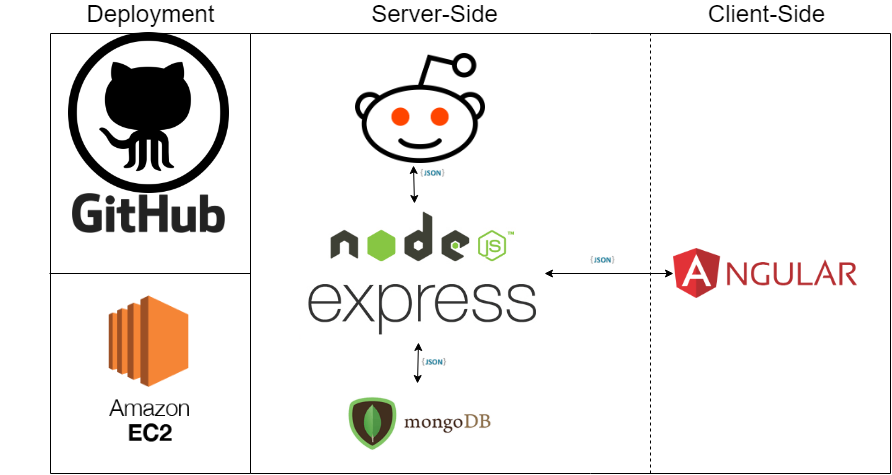
\includegraphics[width=\linewidth]{img/Diagram.png}
  \caption{System Architecture}
  \label{fig:GHP}
\end{figure}

As discussed in section \textit{1.1: Project Objectives}, we will now expand on the system implemented in this project.

\paragraph{Dissertation}
\begin{itemize}
\item Introduce the concept of the project. 
\item Provide an understanding of social media.
\item Provide an understanding of web technologies.
\item Describe the development of the applied project
\end{itemize}
 
 \paragraph{Applied Project}
\begin{itemize}
\item Produce a simple easy to use web application.
\item Deliver a social platform for tech-savvy people that differs from the norm.
\item Dive into new web technologies.
\item Complete the project collaborating as a team using an efficient and effective approach.
\end{itemize}

% ========================== Testing ========================== 
\section{Testing}
It was an important part of the project for us to plan out the project, and test each component of the full stack web development. We started prototyping the MEAN stack as well as developing the project early to test the functionality early.

\subsection{Prototyping}
Early on we built multiple applications to test the functionality of the MEAN stack. We built a Node.js application, then added ExpressJS. Getting a basic grasp of each technology before advancing was very import as to understanding how the system as a whole will work from top to bottom.

\begin{figure}[H]
  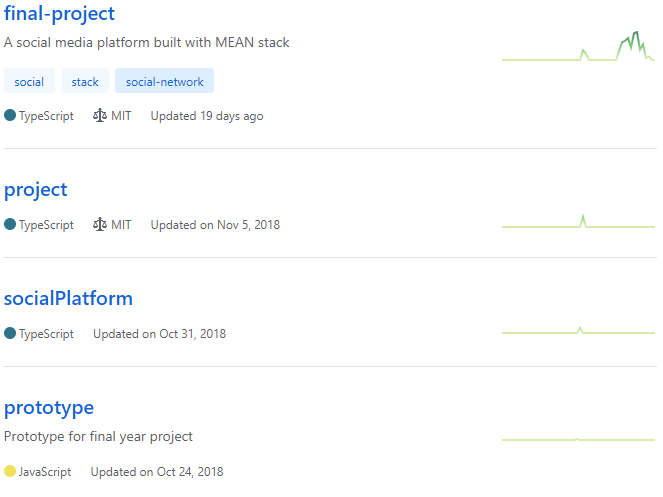
\includegraphics[width=\linewidth]{img/prototypes.PNG}
  \caption{GitHub Prototypes}
  \label{fig:GHP}
\end{figure}

As you can see above there are four GitHub projects. The first one at the top is the final project. The rest are prototypes we developed to test the MEAN stack functionality and understand each component of the MEAN stack (MongoDB, ExpressJS, Node.js, and Angular).

\subsection{Deployment Testing}
We tested the project using a three-stage deployment. Initial, medial and final. Each stage covered certain criteria for the deployment process. Initially used for unit testing, medial for early deployment testing and final for the public release of the application.

\subsubsection{Initial}
Initial testing involved testing the application on the local-host and test each function to see how the application would react to our inputs. This was the primary method of testing individual components and ensuring the application would work on the local-host port 3000.

\subsubsection{Medial}
After the initial testing stage, we had a medial stage for deployment. We built a home server to test the application over a network. This involved buying and building the home server. Once setup and built we connected the PC to the home network and gave the PC a static IP (Internet Protocol). This was extremely important, without giving the server a static IP the local address such as 192.168.0.10 could be moved to 192.168.0.50. If the local IP of the server changed, the port forwarding address would need to change each time the servers did, which would be very tedious. 

Once the IP of the server was setup we port forwarded the port 3000 to the server PC's static IP address. The port 3000 had to be port forwarded because of the application using that port. With this setup, we could access the application from another PC in another location. This was used to demo the application to supervisors in meetings.

\subsubsection{Final}
With a grasp on how deployment works from the stage above we had the knowledge on how and what needed to be done. We deployed our project on AWS (Amazon Web Services). We went with AWS because of their support for the MEAN stack made it a prime contender. Once deployed onto AWS we knew we could access it from inside the instance, but not outside. So knew from above we need to open the port and direct it to our AWS instance. Although in this case, AWS handled the local IP and all we had to do in deployment in this stage was open the port using AWS console, which acted as a router for our AWS instance.

\subsection{Unit Testing}
Unit testing was a testing method we used at every stage in development. Each function block of code was tested for the desired output such as a GET method to the API and then testing to see if that function was retrieving the JSON data before continuing onto the next stage.

\subsection{System Testing}
We used system testing on each stage of deployment to ensure all components worked properly in a deployed environment. This testing method involved using the application and all its components and features. This stage was done far less frequently than unit testing but was just as important to ensure our application was of high quality.

% ========================== Performance ========================== 
\section{Performance}
The application preforms remarkably well. The biggest 'bottleneck' that stifles performance will be the users connection to the program or the service it is hosted on.

The API performs very well, and because of MongoDB using JSON to store data there is no conversion needed, so the computing needed to access the API is very low.

We also used the Reddit API to make news posts and funny posts for users. This API at first was requested by the user when they accessed the home page but quickly realized that when we wanted to add comments and to save posts we would need to store the data in some way. We reformatted how users get the data and realized having the user access an API route that gets the data from the MongoDB was a little bit faster than when we originally set up the application.

The Angular client is extremely responsive and due to its single page, nature felt far more modern than a multiple page website. Angular being a single page web framework allowed our application to have a more modern look and feel to it. As the user changes the view to different components they never see a white screen when changing pages. The navigation bar, for example, is always present when changing views.

% ========================== Objectives ========================== 
\section{Evaluation of Objectives}
In this section we will expand on the objectives we set out for the project. The project was built with these objectives in mind:

\paragraph{Produce a simple easy to use web application:}
We did produce a simple and easy to use web application. Using Node.js to host the application by delivering the Angular application to the user and host the API. Using Angular were were able to compartmentalize each component and work on each individually. Using Angular we were able to provide an easy to navigate and responsive single page web application.

\paragraph{ Deliver a social platform for tech-savvy people that differs from the norm:}
We successfully made a social media platform developed around users who are tech-savvy. The site uses the Reddit API to make sure there is always news posts and funny light-hearted posts based around technology. We also allowed the user to make their own posts to share images and news articles.

We made a comment section to allows a community to built up. Allowing comments was extremely important to allow small developers to put up a post to ask for help and have other users help out. Or a user post a link to their GitHub to ask for their opinion. A comment section had to be nailed down in order to build a community.

To expand on community relations we made user profiles. User profiles allow other users to follow them, see their comments, posts, followed users and subscribed posts. User profiles allow other users to built up a rapport with one another.

We tried to differ from other technology-based social media by adding in funny light-hearted posts from the Reddit API. We felt the only social media available for the tech-savvy were from a much more professional standpoint.

\paragraph{Dive into new web technologies:}
Diving into a new web technology for us was very important. We had experience with Spring, GO and Ruby on  Rails. But we wanted to learn a completely new architecture we had no experience with. After deciding on the MEAN stack, we quickly realized how different web development is with a framework like Angular. Angular as we discussed earlier is a single page web application framework. This was different from the traditional sending an HTML document and having the user interact with that. 

We also had no experience with Node.js. Node.js uses JavaScript which we had quite a lot of experience with, but never outside the browser. Node.js is very powerful and allows developers to do quite a lot very quickly. Node.js includes the Node Package Manager (NPM), which allows developers to access the largest package library. NPM allowed us to considerate on creating function features by using packages such as Passport.js.

\paragraph{Complete  the project collaborating as a team using an efficient and effective approach:}
As a group project and at a scale we've never done before, we wanted to ensure quality and consistency would be kept. We met up weekly to plan out the next stage of development. We also met up with our supervisors weekly to get feedback on our plan and progress made. Using this meeting was extremely important to ensure we were both on the same page.

We also made sure to keep in persistent contact with one another using application such as WhatsApp and Facebook, which allowed us to maintain in contact outside the college. These applications allowed us to share screenshots of errors we both had, and share our thoughts on a feature.

Using GitHub allowed us to both collaborate on a single project and see the changes we were making to the project. Using GitHub branches we could test a feature before committing it to the master branch. GitHub was a great way for us to collaborate on the project together and get a feel for how collaborative projects work.

% ========================== Limitations ========================== 
\section{Limitations and Improvements}
As the project developed and we got more and more experience with the MEAN architecture, we came up with better methods of developing features. 

\subsection{Server}
As became more experienced with Node.js and its available packages, we realized better methods of using developing the API and retrieving data from the Reddit API. One example of an improvement we would do if we developed another API service is to use swagger from the beginning. As we developed an API service we created routes that would return a specific amount of posts for example. And a route that would return all posts. What we should have done is create a route for posts and send a number of posts I want. This could also be said for comments, such as sending how many I want and from what commenter I want them, rather than create a set route for sending a username that would return a set amount.

\subsection{Client}
As we got better at developing with Angular we improved elements of how data is displayed from the server. Early on we used tables to display the posts and later moved to Angular Material. One thing we would have liked to introduce to the social media site is user tags. We would have liked to add a tag to themselves to show the position they hold in the industry so other users can gauge their ability. Such as 'Cian<Software Student 4 years>', so other users can see how experienced they are and take their feedback into account.


% ========================== Overall Evaluation ========================== 
\section{Overall Evaluation}
Overall the system works as indented and functions as an effective social media tool. It met the requirements set out in section 1.1 Project Objectives and went beyond what we originally set. Based on the tests we carried out throughout the project with prototypes and unit tests we were able to build an effective application and find and fix any bugs throughout development. Prototyping was an important phase which helped up understand the MEAN stack on an individual component level. The MEAN stack architecture proved very reliable and easy to develop for. Although we could have improved and added more components to the application we were overall very happy with the progress we made.
